


\tikzset{every picture/.style={line width=0.75pt}} %set default line width to 0.75pt        

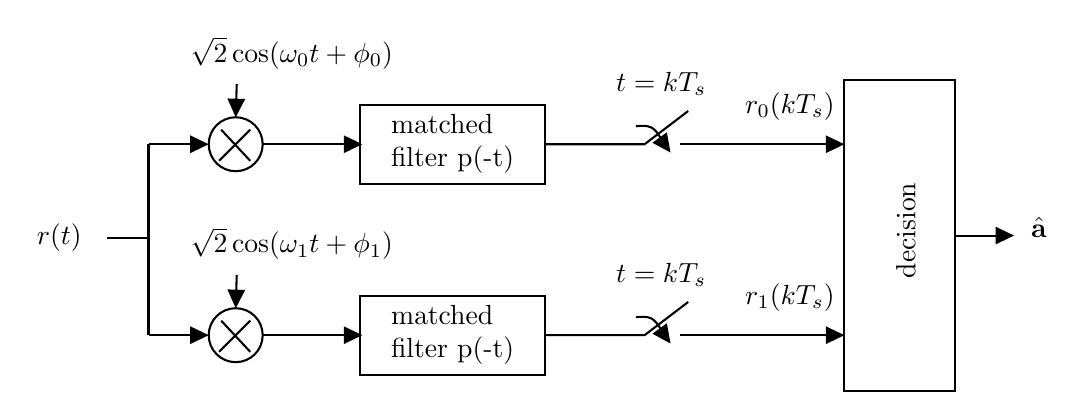
\begin{tikzpicture}[x=0.75pt,y=0.75pt,yscale=-1,xscale=1]
%uncomment if require: \path (0,378); %set diagram left start at 0, and has height of 378

%Straight Lines [id:da015204313020472648] 
\draw    (100,127) -- (120,127) ;
%Straight Lines [id:da3807433535655065] 
\draw    (120,174) -- (120,82) ;
%Straight Lines [id:da13452699900895748] 
\draw    (120,82) -- (146,82) ;
\draw [shift={(149,82)}, rotate = 180] [fill={rgb, 255:red, 0; green, 0; blue, 0 }  ][line width=0.08]  [draw opacity=0] (8.93,-4.29) -- (0,0) -- (8.93,4.29) -- cycle    ;
%Shape: Rectangle [id:dp6831503614766208] 
\draw   (222,63) -- (311,63) -- (311,101) -- (222,101) -- cycle ;
%Shape: Circle [id:dp5132093237924611] 
\draw   (149,82) .. controls (149,74.82) and (154.82,69) .. (162,69) .. controls (169.18,69) and (175,74.82) .. (175,82) .. controls (175,89.18) and (169.18,95) .. (162,95) .. controls (154.82,95) and (149,89.18) .. (149,82) -- cycle ;
%Straight Lines [id:da25287195023205933] 
\draw    (155,75) -- (169,90) ;
%Straight Lines [id:da5242592168562576] 
\draw    (169,75) -- (154,90) ;
%Straight Lines [id:da23051729614765581] 
\draw    (162.09,66) -- (162.5,53) ;
\draw [shift={(162,69)}, rotate = 271.79] [fill={rgb, 255:red, 0; green, 0; blue, 0 }  ][line width=0.08]  [draw opacity=0] (8.93,-4.29) -- (0,0) -- (8.93,4.29) -- cycle    ;
%Straight Lines [id:da2971482914437682] 
\draw    (175,82) -- (220,82) ;
\draw [shift={(223,82)}, rotate = 180] [fill={rgb, 255:red, 0; green, 0; blue, 0 }  ][line width=0.08]  [draw opacity=0] (8.93,-4.29) -- (0,0) -- (8.93,4.29) -- cycle    ;
%Straight Lines [id:da24289517343868772] 
\draw    (311,82) -- (359,82) -- (380,66) ;
%Straight Lines [id:da03913348203652922] 
\draw    (376,82) -- (452.24,82) ;
\draw [shift={(455.24,82)}, rotate = 180] [fill={rgb, 255:red, 0; green, 0; blue, 0 }  ][line width=0.08]  [draw opacity=0] (8.93,-4.29) -- (0,0) -- (8.93,4.29) -- cycle    ;
%Curve Lines [id:da6656366911860763] 
\draw    (354.83,73.33) .. controls (364.08,72.41) and (363.64,74.62) .. (369.85,83.66) ;
\draw [shift={(371.5,86)}, rotate = 233.97] [fill={rgb, 255:red, 0; green, 0; blue, 0 }  ][line width=0.08]  [draw opacity=0] (8.93,-4.29) -- (0,0) -- (8.93,4.29) -- cycle    ;
%Shape: Rectangle [id:dp38931328167896195] 
\draw   (455.24,51) -- (508.5,51) -- (508.5,201) -- (455.24,201) -- cycle ;
%Straight Lines [id:da5073149386864682] 
\draw    (508,126) -- (534,126) ;
\draw [shift={(537,126)}, rotate = 180] [fill={rgb, 255:red, 0; green, 0; blue, 0 }  ][line width=0.08]  [draw opacity=0] (8.93,-4.29) -- (0,0) -- (8.93,4.29) -- cycle    ;
%Straight Lines [id:da0935600260327849] 
\draw    (120,174) -- (146,174) ;
\draw [shift={(149,174)}, rotate = 180] [fill={rgb, 255:red, 0; green, 0; blue, 0 }  ][line width=0.08]  [draw opacity=0] (8.93,-4.29) -- (0,0) -- (8.93,4.29) -- cycle    ;
%Shape: Rectangle [id:dp5397600807528802] 
\draw   (222,155) -- (311,155) -- (311,193) -- (222,193) -- cycle ;
%Shape: Circle [id:dp6340079603545306] 
\draw   (149,174) .. controls (149,166.82) and (154.82,161) .. (162,161) .. controls (169.18,161) and (175,166.82) .. (175,174) .. controls (175,181.18) and (169.18,187) .. (162,187) .. controls (154.82,187) and (149,181.18) .. (149,174) -- cycle ;
%Straight Lines [id:da054936665320719724] 
\draw    (155,167) -- (169,182) ;
%Straight Lines [id:da14446384117365363] 
\draw    (169,167) -- (154,182) ;
%Straight Lines [id:da06806069680494597] 
\draw    (162.09,158) -- (162.5,145) ;
\draw [shift={(162,161)}, rotate = 271.79] [fill={rgb, 255:red, 0; green, 0; blue, 0 }  ][line width=0.08]  [draw opacity=0] (8.93,-4.29) -- (0,0) -- (8.93,4.29) -- cycle    ;
%Straight Lines [id:da13918324188613052] 
\draw    (175,174) -- (220,174) ;
\draw [shift={(223,174)}, rotate = 180] [fill={rgb, 255:red, 0; green, 0; blue, 0 }  ][line width=0.08]  [draw opacity=0] (8.93,-4.29) -- (0,0) -- (8.93,4.29) -- cycle    ;
%Straight Lines [id:da7726545291977289] 
\draw    (311,174) -- (359,174) -- (380,158) ;
%Straight Lines [id:da5999576449313313] 
\draw    (376,174) -- (452.24,174) ;
\draw [shift={(455.24,174)}, rotate = 180] [fill={rgb, 255:red, 0; green, 0; blue, 0 }  ][line width=0.08]  [draw opacity=0] (8.93,-4.29) -- (0,0) -- (8.93,4.29) -- cycle    ;
%Curve Lines [id:da38919606803399187] 
\draw    (354.83,165.33) .. controls (364.08,164.41) and (363.64,166.62) .. (369.85,175.66) ;
\draw [shift={(371.5,178)}, rotate = 233.97] [fill={rgb, 255:red, 0; green, 0; blue, 0 }  ][line width=0.08]  [draw opacity=0] (8.93,-4.29) -- (0,0) -- (8.93,4.29) -- cycle    ;

% Text Node
\draw (189,38) node    {$\sqrt{2}\cos( \omega _{0} t+\phi _{0})$};
% Text Node
\draw (266.5,82) node   [align=left] {matched\\filter p(-t)};
% Text Node
\draw (367,53) node    {$t=kT_{s}$};
% Text Node
\draw (429,64) node    {$r_{0}( kT_{s})$};
% Text Node
\draw (484.87,123.5) node  [rotate=-269.97] [align=left] {decision};
% Text Node
\draw (549,122) node    {$\hat{\mathbf{a}}$};
% Text Node
\draw (77,127) node    {$r( t)$};
% Text Node
\draw (189,130) node    {$\sqrt{2}\cos( \omega _{1} t+\phi _{1})$};
% Text Node
\draw (266.5,174) node   [align=left] {matched\\filter p(-t)};
% Text Node
\draw (367,145) node    {$t=kT_{s}$};
% Text Node
\draw (429,156) node    {$r_{1}( kT_{s})$};


\end{tikzpicture}